\documentclass{article}

\usepackage{hyperref}
\hypersetup{
	colorlinks=true,
	linkcolor=blue,
	urlcolor=cyan,}
\usepackage{booktabs}
\usepackage{textgreek}

%%%%%%%%%%%%%%%%%%%%%%%%%%%%%%%%%%%%%%%%%
% Lachaise Assignment
% Structure Specification File
% Version 1.0 (26/6/2018)
%
% This template originates from:
% http://www.LaTeXTemplates.com
%
% Authors:
% Marion Lachaise & François Févotte
% Vel (vel@LaTeXTemplates.com)
%
% License:
% CC BY-NC-SA 3.0 (http://creativecommons.org/licenses/by-nc-sa/3.0/)
% 
%%%%%%%%%%%%%%%%%%%%%%%%%%%%%%%%%%%%%%%%%

%----------------------------------------------------------------------------------------
%	PACKAGES AND OTHER DOCUMENT CONFIGURATIONS
%----------------------------------------------------------------------------------------

\usepackage{amsmath,amsfonts,stmaryrd,amssymb} % Math packages

\usepackage{enumerate} % Custom item numbers for enumerations

\usepackage[ruled]{algorithm2e} % Algorithms

\usepackage[framemethod=tikz]{mdframed} % Allows defining custom boxed/framed environments

\usepackage{listings} % File listings, with syntax highlighting
\lstset{
	basicstyle=\ttfamily, % Typeset listings in monospace font
}

%----------------------------------------------------------------------------------------
%	DOCUMENT MARGINS
%----------------------------------------------------------------------------------------

\usepackage{geometry} % Required for adjusting page dimensions and margins

\geometry{
	paper=a4paper, % Paper size, change to letterpaper for US letter size
	top=2.5cm, % Top margin
	bottom=3cm, % Bottom margin
	left=2.5cm, % Left margin
	right=2.5cm, % Right margin
	headheight=14pt, % Header height
	footskip=1.5cm, % Space from the bottom margin to the baseline of the footer
	headsep=1.2cm, % Space from the top margin to the baseline of the header
	%showframe, % Uncomment to show how the type block is set on the page
}

%----------------------------------------------------------------------------------------
%	FONTS
%----------------------------------------------------------------------------------------

\usepackage[utf8]{inputenc} % Required for inputting international characters
\usepackage[T1]{fontenc} % Output font encoding for international characters

\usepackage{XCharter} % Use the XCharter fonts

%----------------------------------------------------------------------------------------
%	COMMAND LINE ENVIRONMENT
%----------------------------------------------------------------------------------------

% Usage:
% \begin{commandline}
%	\begin{verbatim}
%		$ ls
%		
%		Applications	Desktop	...
%	\end{verbatim}
% \end{commandline}

\mdfdefinestyle{commandline}{
	leftmargin=10pt,
	rightmargin=10pt,
	innerleftmargin=15pt,
	middlelinecolor=black!50!white,
	middlelinewidth=2pt,
	frametitlerule=false,
	backgroundcolor=black!5!white,
	frametitle={Command Line},
	frametitlefont={\normalfont\sffamily\color{white}\hspace{-1em}},
	frametitlebackgroundcolor=black!50!white,
	nobreak,
}

% Define a custom environment for command-line snapshots
\newenvironment{commandline}{
	\medskip
	\begin{mdframed}[style=commandline]
}{
	\end{mdframed}
	\medskip
}

%----------------------------------------------------------------------------------------
%	FILE CONTENTS ENVIRONMENT
%----------------------------------------------------------------------------------------

% Usage:
% \begin{file}[optional filename, defaults to "File"]
%	File contents, for example, with a listings environment
% \end{file}

\mdfdefinestyle{file}{
	innertopmargin=1.6\baselineskip,
	innerbottommargin=0.8\baselineskip,
	topline=false, bottomline=false,
	leftline=false, rightline=false,
	leftmargin=2cm,
	rightmargin=2cm,
	singleextra={%
		\draw[fill=black!10!white](P)++(0,-1.2em)rectangle(P-|O);
		\node[anchor=north west]
		at(P-|O){\ttfamily\mdfilename};
		%
		\def\l{3em}
		\draw(O-|P)++(-\l,0)--++(\l,\l)--(P)--(P-|O)--(O)--cycle;
		\draw(O-|P)++(-\l,0)--++(0,\l)--++(\l,0);
	},
	nobreak,
}

% Define a custom environment for file contents
\newenvironment{file}[1][File]{ % Set the default filename to "File"
	\medskip
	\newcommand{\mdfilename}{#1}
	\begin{mdframed}[style=file]
}{
	\end{mdframed}
	\medskip
}

%----------------------------------------------------------------------------------------
%	NUMBERED QUESTIONS ENVIRONMENT
%----------------------------------------------------------------------------------------

% Usage:
% \begin{question}[optional title]
%	Question contents
% \end{question}

\mdfdefinestyle{question}{
	innertopmargin=1.2\baselineskip,
	innerbottommargin=0.8\baselineskip,
	roundcorner=5pt,
	nobreak,
	singleextra={%
		\draw(P-|O)node[xshift=1em,anchor=west,fill=white,draw,rounded corners=5pt]{%
		Question \theQuestion\questionTitle};
	},
}

\newcounter{Question} % Stores the current question number that gets iterated with each new question

% Define a custom environment for numbered questions
\newenvironment{question}[1][\unskip]{
	\bigskip
	\stepcounter{Question}
	\newcommand{\questionTitle}{~#1}
	\begin{mdframed}[style=question]
}{
	\end{mdframed}
	\medskip
}

%----------------------------------------------------------------------------------------
%	WARNING TEXT ENVIRONMENT
%----------------------------------------------------------------------------------------

% Usage:
% \begin{warn}[optional title, defaults to "Warning:"]
%	Contents
% \end{warn}

\mdfdefinestyle{warning}{
	topline=false, bottomline=false,
	leftline=false, rightline=false,
	nobreak,
	singleextra={%
		\draw(P-|O)++(-0.5em,0)node(tmp1){};
		\draw(P-|O)++(0.5em,0)node(tmp2){};
		\fill[black,rotate around={45:(P-|O)}](tmp1)rectangle(tmp2);
		\node at(P-|O){\color{white}\scriptsize\bf !};
		\draw[very thick](P-|O)++(0,-1em)--(O);%--(O-|P);
	}
}

% Define a custom environment for warning text
\newenvironment{warn}[1][Warning:]{ % Set the default warning to "Warning:"
	\medskip
	\begin{mdframed}[style=warning]
		\noindent{\textbf{#1}}
}{
	\end{mdframed}
}

%----------------------------------------------------------------------------------------
%	INFORMATION ENVIRONMENT
%----------------------------------------------------------------------------------------

% Usage:
% \begin{info}[optional title, defaults to "Info:"]
% 	contents
% 	\end{info}

\mdfdefinestyle{info}{%
	topline=false, bottomline=false,
	leftline=false, rightline=false,
	nobreak,
	singleextra={%
		\fill[black](P-|O)circle[radius=0.4em];
		\node at(P-|O){\color{white}\scriptsize\bf i};
		\draw[very thick](P-|O)++(0,-0.8em)--(O);%--(O-|P);
	}
}

% Define a custom environment for information
\newenvironment{info}[1][Info:]{ % Set the default title to "Info:"
	\medskip
	\begin{mdframed}[style=info]
		\noindent{\textbf{#1}}
}{
	\end{mdframed}
}
 % Include the file specifying the document structure and custom commands

%----------------------------------------------------------------------------------------
%	ASSIGNMENT INFORMATION
%----------------------------------------------------------------------------------------

\title{Week 2: Electromyography (EMG) I}
\author{BIOE 320 Systems Physiology Laboratory} 
\date{}
%----------------------------------------------------------------------------------------

\begin{document}
\large
\maketitle

\section*{Objectives}
\begin{enumerate}
	\item To record and compare maximum clench strengths for dominant and non-dominant arms using the BIOPAC system
	\item To record and compare skeletal muscle tonus measurements in dominant and non-dominant arms
	\item To record, analyze, and explain EMG signals for several daily activities
\end{enumerate}

\section*{Background}
Muscles convert chemical energy into mechanical work. The mechanical work
achieved by muscles is called a contraction. Muscle contractions occur after an action potential is sent from the brain to motor neurons which chemically signal the desired muscle fibers to contract. The motor neuron and all the associated muscle fibers that control the contraction and relaxation of a specific muscle are collectively called \textbf{motor unit} (Fig. \ref{motor_unit}).

\begin{figure}[h]
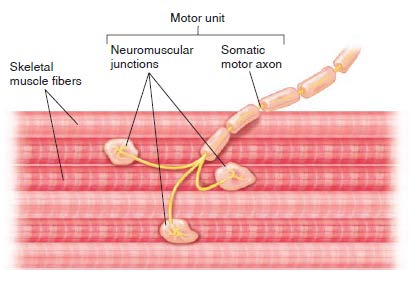
\includegraphics[width=0.5\textwidth]{../images/EMG_I_1.jpg}
\centering
\caption{Motor unit.}
\label{motor_unit}
\end{figure}

\subsection*{Motor Unit Recruitment}

\begin{figure}[h]
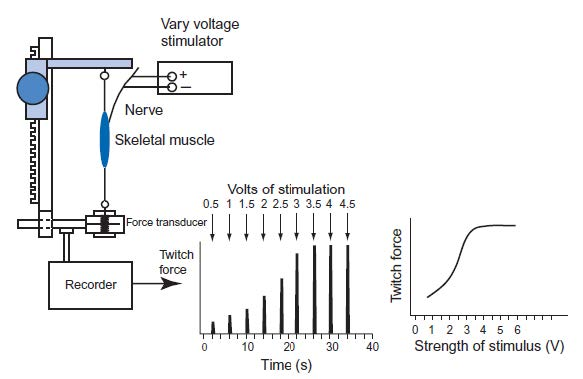
\includegraphics[width=0.8\textwidth]{../images/EMG_I_2.jpg}
\centering
\caption{Increase in the muscle twitch force via the increased recruitment of motor fibers by increasing the strength of the external stimulus.}
\label{force}
\end{figure}

The strength of muscle contractions can be modulated through two primary methods. The first method (spatial summation) occurs through the gradual \textbf{recruitment of motor units}, as shown in Fig. \ref{force}. The body recruits its weakest (smallest) motor units first, and successively recruits stronger (larger) motor units until the desired force is achieved. Motor unit size is defined by the number of muscle fibers to which a motor neuron is connected. Large motor units have thousands of muscle fibers, while small motor units may have as little as ten muscle fibers. Small muscle fibers are typically utilized for activities that require high precision.

\begin{figure}[h]
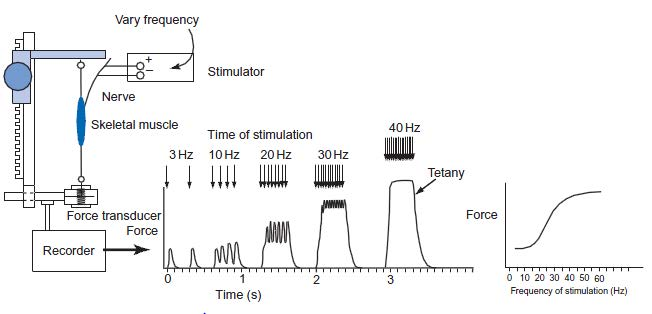
\includegraphics[width=0.8\textwidth]{../images/EMG_I_3.jpg}
\centering
\caption{Increasing the frequency of stimulation at low frequencies only increases the frequency of the same twitch wave form. When the period of the stimulation frequency is shorter than the period of the twitch, force begins to summate.}
\label{freq}
\end{figure}

The second factor (temporal summation) contributing to the magnitude of muscle contraction is the \textbf{rate of firing}. By increasing action potential firing rate, the amount of time the muscle fibers have to relax is decreased, and thus the incremental forces produced from each muscle fiber contraction accumulate to a greater force, as shown in Fig. \ref{freq}. An increase in action potential frequency that results in a state of sustained muscular contractions without periods of relaxation of the muscle fibers, is called \textbf{tetanus}.

\subsection*{Muscle Tone (Tonus)}
Muscle tone is the partial contractile state muscles maintain in order to preserve the structural integrity of all of the body’s organs and extremities. Although we will be dealing only with skeletal muscles in this lab, cardiac and smooth muscles also possess a level of tone which functions to maintain structural integrity and to control pressures and flow of bodily fluids.

\section*{Experimental Methods}
\subsection*{Setting Up the Software}
\begin{enumerate}
	\item Open BIOPAC student lab lessons software and select \textit{L01 - Electromyography (EMG) I} (Fig. \ref{lesson}).
		\begin{figure}[h]
	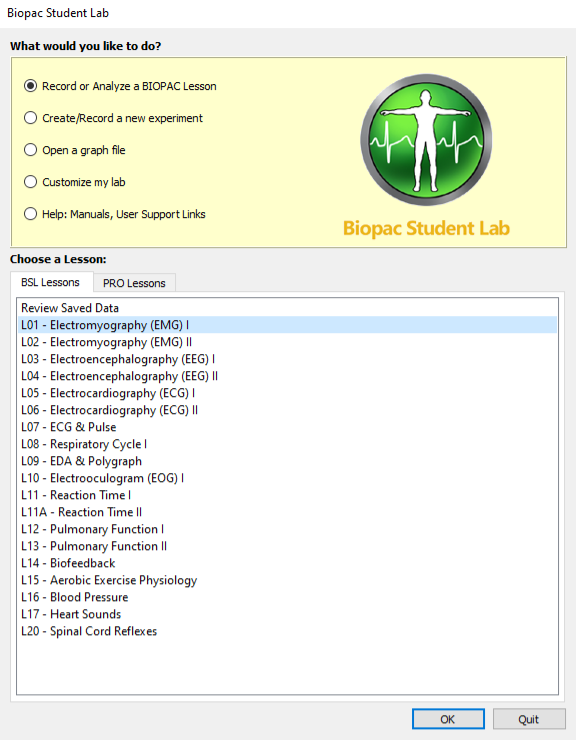
\includegraphics[width=0.6\textwidth]{../images/EMG_I_13.png}
		\centering
		\caption{Selecting BIOPAC lesson L01}
		\label{lesson}
		\end{figure}
		
	\item When the prompt asking for your file name appears, name the file using your name and a description about the lab (e.g. "\textit{FirstnameLastname\_EMG\_I}"). The BIOPAC student software will create a folder to store your data files.
	\item Follow the instructions on-screen, which will indicate which channel you should plug in your electrode lead. For most units, this will be channel 1.	
	\item Plug your electrode leads into the indicated channel on the MP3X as shown in Fig. \ref{channel2}.
		\begin{figure}[h]
	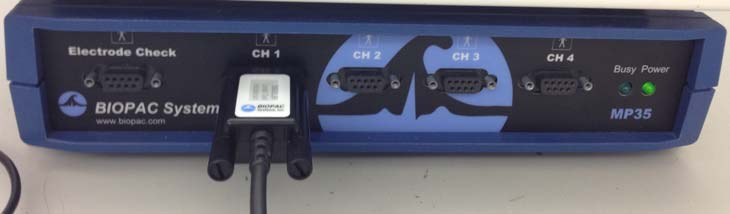
\includegraphics[width=0.8\textwidth]{../images/EMG_I_6.jpg}
		\centering
		\caption{Physical location of MP3X channels.}
		\label{channel2}
		\end{figure}
	
	\item Select a subject for EMG measurements. Follow the instructions on-screen for subject setup.
		\begin{itemize}
			\item Red (+): closer to wrist
			\item White (-): closer to elbow
			\item Black (ground): wrist bone
		\end{itemize}
	\item For the first recording segment, choose the subject's dominant arm to attach the leads. This will be Forearm 1.
	\item Follow the instruction on-screen to calibrate.
\end{enumerate}

\subsection*{Data Acquisition}
You will record two segments of data per subject: one segment for Forearm 1 (the dominant arm), and one segment for Forearm 2 (the non-dominant arm).
\begin{enumerate}
	\item When you begin to record, the subject will repeat a cycle of clench-release-wait as follows: clench hand, hold the clench for 2 seconds, release the clench, and wait for 2 seconds before beginning the next clench cycle.
	\item The subject will record 4 clench-release-wait cycles as described above. Clench strength should be increased for each following cycle in equal increments, doubling the clench strength for each cycle. The fourth clench strength should be the subject's maximum clench strength.
	\item When you are ready, click \textit{Record} and begin collecting data. After the fourth clench, click \textit{Suspend.} If your data does not resemble the example on-screen, click \textit{Redo} to repeat the process.
	\item Attach the electrodes to the subject's non-dominant arm (Forearm 2).
	\item Click \textit{Record} and repeat the same clench-release-wait cycle as was performed for the dominant arm. The BIOPAC program will automatically insert a marker labeled "forearm 2" in the marker bar.
	\item After you have finished measurements for both forearms, you may remove the electrodes from both arms.
	\item Click \textit{Stop} in the upper left hand corner of your screen to finish recording. A dialog box will appear asking if you are finished with your recordings. Click \textit{Yes} to end the data recording and save the data.
	\item If a dialog box pops up, you can listen to the EMG signal (optional, ask the instructor for headphones). When you are finished, click \textit{Stop}. A box will then appear; select \textit{Stop}, then \textit{Analyze Current Data File}, and proceed with the lab.
\end{enumerate}

\section*{Data Analysis}
\begin{enumerate}
	\item The first marker indicates the beginning of Forearm 1 data, and the second marker indicates the beginning of Forearm 2 data. For most units, channel 1 displays the standard EMG data; if you plugged in your electrodes to channel 3, standard EMG data will be displayed on channel 3.
	\item Channel 40 displays the integrated EMG data, which is similar to the absolute value of the EMG. It appears to "trace" an imaginary upper edge of the standard EMG signal as shown in Fig. \ref{integrated}.
		\begin{figure}[h]
	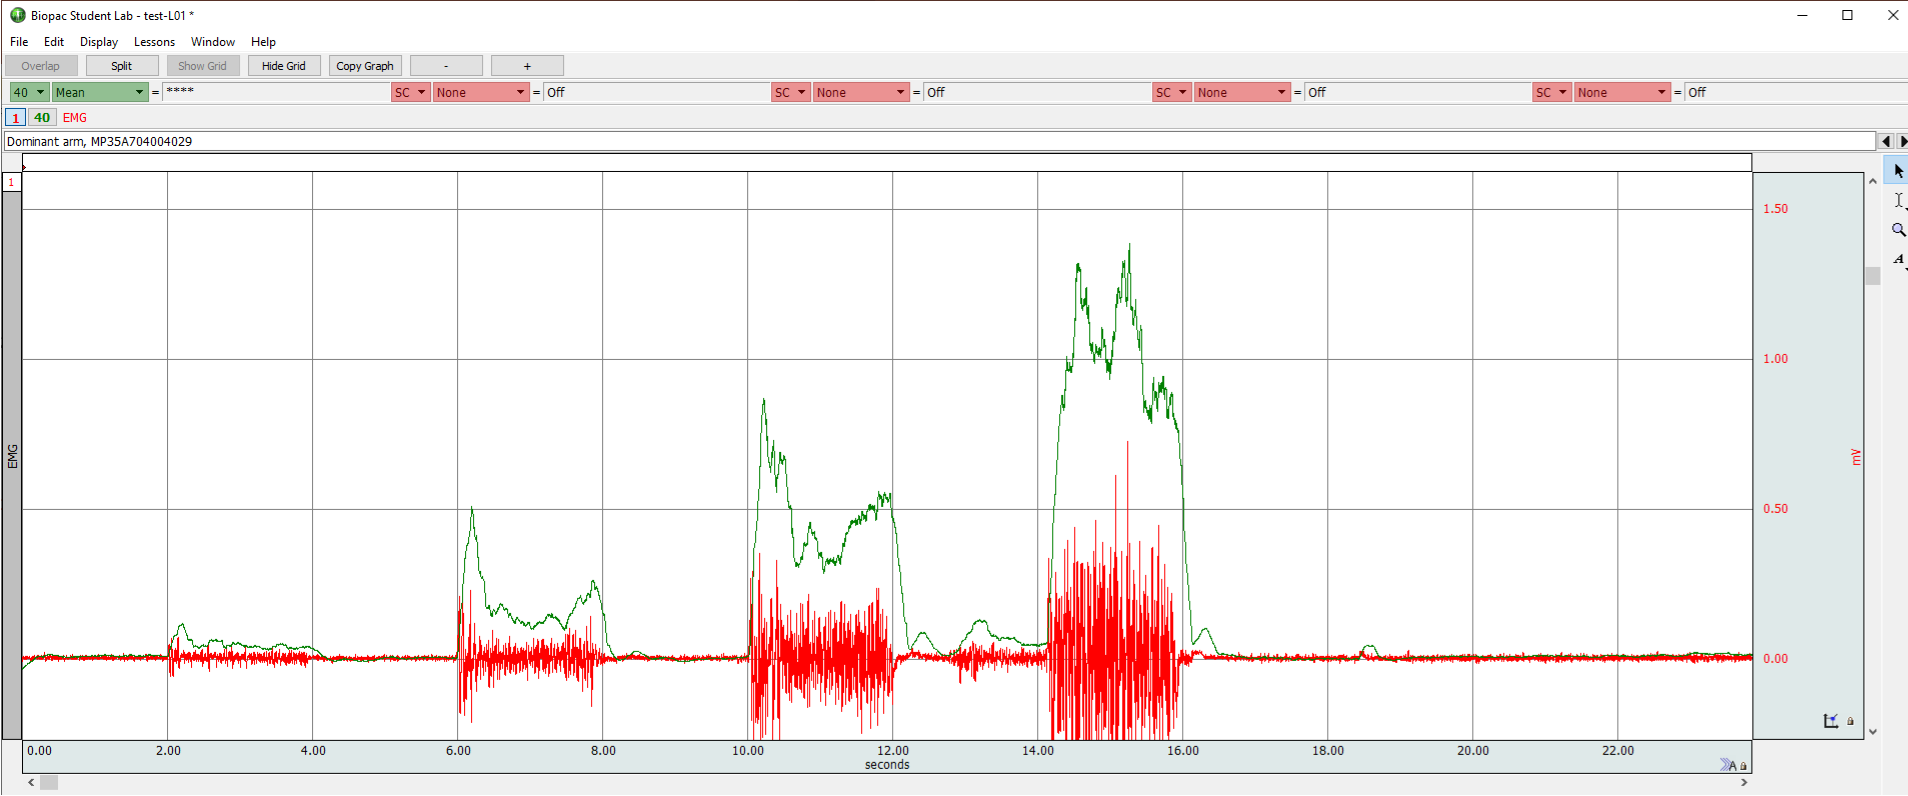
\includegraphics[width=0.8\textwidth]{../images/EMG_I_15.png}	
		\centering
		\caption{Integrated EMG overlapped with standard EMG.}
		\label{integrated}
		\end{figure}

	\item Scale your data so that you can view the first four clusters of standard EMG signal.
	\item Set up the following measurement boxes:
		\begin{table}[h!]
	\centering
	\label{meas_boxes}
	\begin{tabular}[h!]{cc}
	\toprule
	Channel & Measurement\\
	\midrule
	1 & Min\\
	1 & Max\\
	1 & P-P\\
	40 & Mean\\
	\bottomrule
	\end{tabular}
	\end{table}
	
	\item Use the I-beam tool to select one EMG cluster at a time. Use the "plateau" region of the integrated EMG to guide your selection, and avoid highlighting the "build up" EMG signals of your desired contraction (Fig. \ref{highlighting})
		\begin{figure}[h]
	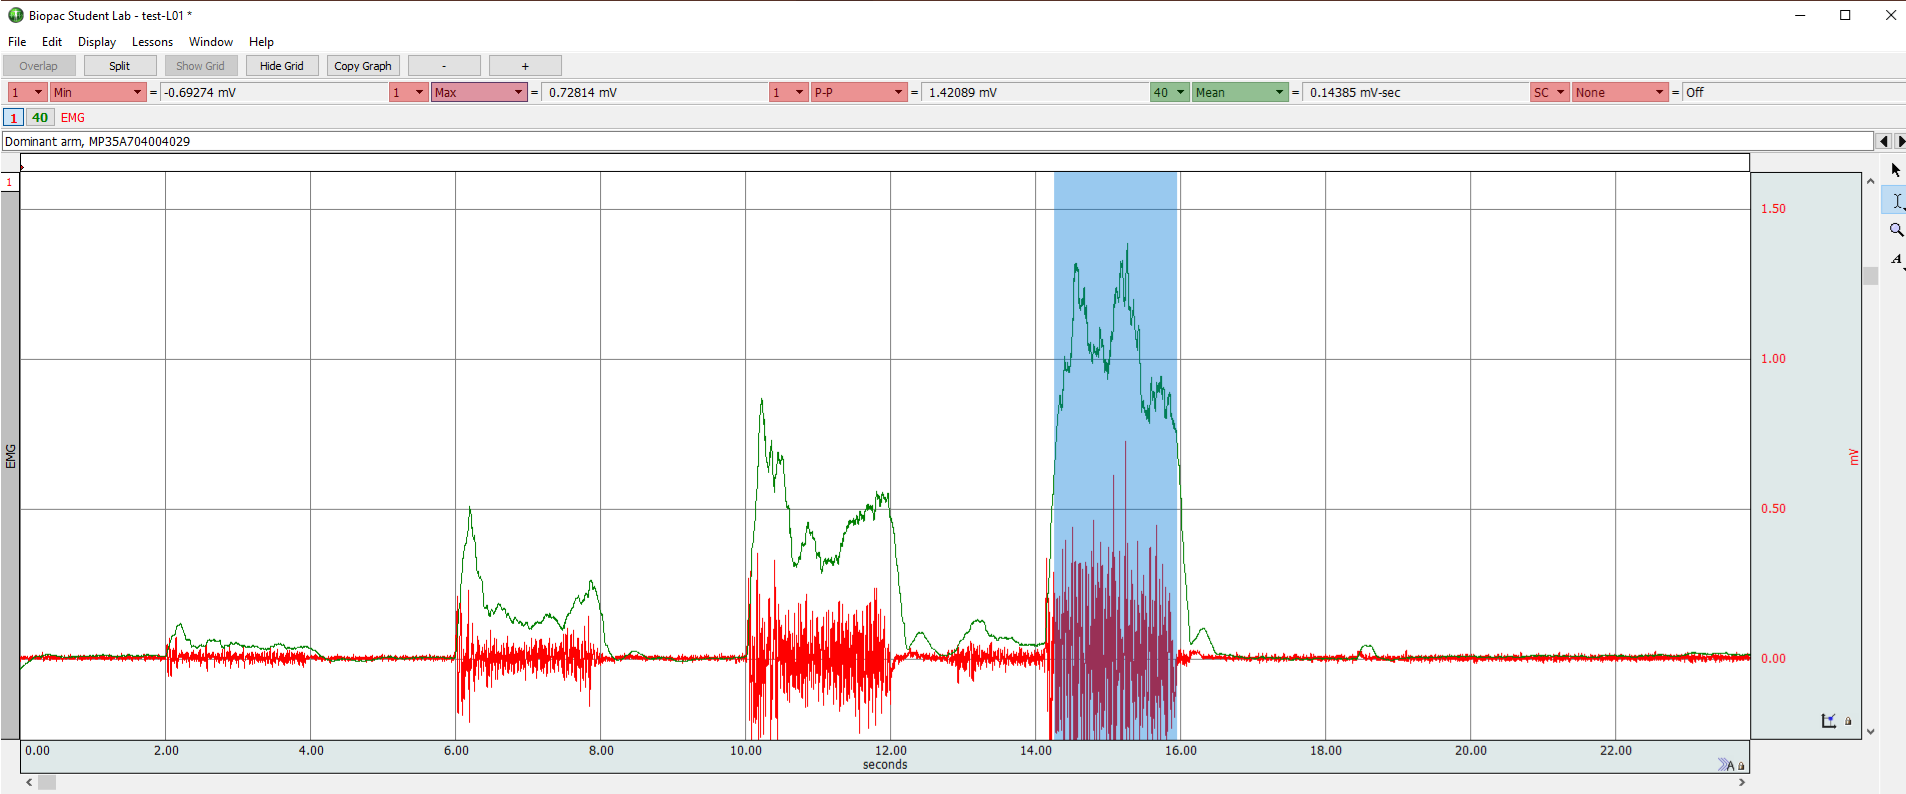
\includegraphics[width=0.8\textwidth]{../images/EMG_I_16.png}	
		\centering
		\caption{Highlighting EMG peaks.}
		\label{highlighting}
		\end{figure}
	
	\item Record your measurement values for Forearm 1 (dominant arm) on your handout.
	\begin{enumerate}
		\item What is the percentage increase or decrease in EMG activity between the weakest and strongest clench for the dominant forearm? Show your calculations.
		\item Why can't you use the raw EMG signal to determine the mean value? Why must the integrated EMG signal be used?
	\end{enumerate}
	\item Repeat the measurement process for Forearm 2 (non-dominant arm) and record the values on your handout.
	\begin{enumerate}
		\item Compare the mean values of the strongest clench in EMG activity between the two forearms. Report the difference between the two forearms as a magnitude (mV or mV-sec) as well as a percentage (\%). Show your calculations.
		\item Does the dominant or non-dominant forearm show the highest EMG clench? Explain the physiological basis of your results.
		\item List four factors that influence maximum clench strength.
	\end{enumerate}
	
	\item Measure tonus by examining the periods of rest in between each EMG cluster. While acquiring these values, be careful to only collect tonus data, i.e. do not use any measurements where clenching is taking place. Record these values on your handout.
	\begin{enumerate}
		\item Is there a difference in tonus between the two forearms? If so, quantify (and show your work) and explain why.
	\end{enumerate}
	\item You may close and save the current BIOPAC recording.
\end{enumerate}
\end{document}
